%%DESCRIBE LO, NLO, ect
%%DESCRIBE POWHEG
\chapter{Event and Detector Simulation}
Event simulation is crucial
in order to measure detector acceptances and efficiencies 
for various physics processes and to estimate backgrounds 
due to known but SM physics processes. 
Event simulation requires
prediction of a physics process expected at the LHC, production
of physics final states and distribution in phase space of final state particles
and then simulation of particle interactions within the detector\cite{Buckley:2011ms}. %%fix
The physics process is simulated using a monte carlo (MC) generator
while the simulation of the detector is performed using a dedicated
software package which models in interactions of particles
in their passage through matter.  
The output of simulation should be similar if not the same as
the output of the detector; in this way the simulation and data can undergo the
same reconstruction and analysis.
Simulations are initiated using a program called an 'event generator'.
The purpose of an event generator is to produce hypothetical
events with a distribution of observables as predicted by theory.
%simulated in geant4
%They can then be handed to a detector simulator such as Geantfour
%what is an event generator
%need more here
Event simulation can be used for the following:
\begin{itemize}
\item Aid in the design of detectors and experiments.
\item Provide a prediction 
of what physics processes can be expected and at what rates
\item As a tool for devising analysis strategies to optimize signal significance and
reduce unwanted backgrounds.
\item As a framework to in which to test signal significance.
\item As a means to test current physics theory/model and aid in the confirmation of new physics discovery.
\end{itemize}
In the study of particle physics it is important to not 
trust completely a single generator; if particle physics where perfectly
understood and well modeled then there would be no point in building a detector! 
Instead, it is important to understand the ingredients that go into 
a simulation and choose a generator which describes well the desired process. 
A number of physics generators
are in common use; a few of these are outlined in section \ref{sec:MCGenerators}.
Physics simulation can be divided into a few key components:
The hard scattering matrix elements, which define the process(es) under study,
the structure function, which models the momentum distributions of the partons
which are involved in the collision, final and initial state radiation and underlying
event processes including multiple interactions in the detector.
%\section{Physics Event Generation}
\section{Hard Scattering Process}
Hard scattering matrix element generation of a hard scattering process 
begins typically with a well defined subprocess.
Considering the simulation of 
the process $W\rightarrow\mu\nu$ we start with the leading order differential cross section defined as,  
\begin{equation}
d\sigma(\bar{q}q'\rightarrow W^{-}\rightarrow \mu^{-}\bar{\nu_{\mu}})
=f(x,\mu_{F})f'(x',\mu_{F})\frac{1}{2\hat{s}}|\mathcal{M}(\bar{q}q'\rightarrow W^{-}\rightarrow \mu^{-}\bar{\nu_{\mu}})|^{2}
\frac{d\cos\theta d\phi}{8(2\pi)^{2}}
\label{eq:matrixEle}
\end{equation}
%subject to the kinematic constraint that x1x2S=s where S 
%and s are the collider and subprocess centre of-mass energies-squared respectively
where the decay angles $(\theta,\phi)$ of the $W^{-}$ are two degrees of
freedom. $\mathcal{M}$ is the relevant matrix element, 
$q$ and $q'$ are the initial partons,
$1/(2\hat{s})$ is the parton flux and
 $\hat{s}=xx's$ where $s$ is the center of mass energy squared.
The factorization scale is $\mu_{F}$ and has the physical 
interpertation as a collinear cutoff\cite{Maltoni:2007tc}.  
%In typical event generators which simulate hard processes 
%ref equation
Equation (\ref{eq:matrixEle}) is used to write an event generator. 
To do this first a sampling of the relevant phase
space must be performed using a random number generator which selects
momenta of the colliding constituents by sampling
the parton distribution function of the proton at the energy scale
of the subprocess.

Next, the events must be unweighted using the hit-and-miss 
technique to produce events with observables. %%this is terrible, fix later? jan 8th
The relevant phase space for this process is two dimensional: -1 $< \cos\theta <$ 1,
0 $< \phi < $ 2$\pi$. The values of $cos\theta$ and $\phi$ can be chosen using
a uniform random number generator. 
Evaluating the equation (\ref{eq:matrixEle}) at $d\sigma(\theta_{i},\phi_{i})$ gives
that candidate event's differential cross section which is equivalent to the 
probability of this event occurring. The average of many candidate event's differential
cross section, $\langle d\sigma\rangle$, is an approximation to $\int d\sigma$ and converges
to the measured cross section.
So far, the candidate events are distributed flat in phase space and there is 
no physics information in the distributions.
The next step then is to unweight the event using the 'hit-and-miss' technique
so that they are distributed according to theoretical prediction. By unweighting
the events are generated with the frequency predicted by the theory 
being modeled and individual events represent what might be observed in a
trial experiment. 

%Parton Distribution Functions
%Parton Showering and Hadronization
\subsection{Parton Showering, Hadronization and the Underlying Event}
To successfully simulate a process in a hadron hadron collider the simulated event must include 
parton showering, hadronization and simulation of the underlying event.
Parton showering is a form of correction to the hard scattering subprocess
where it is not feasible to calculate these processes exactly.
Programs that use the parton shower approach are also
able to simulate a wide variety of initial and final state processes.

\begin{figure}[hb]
  \centering
	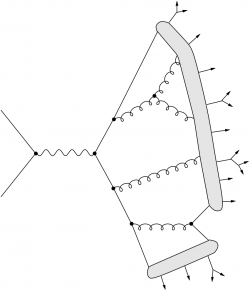
\includegraphics[width=0.5\textwidth]{images/stringModel.png}
  	\caption[Lund String Model for Parton Showering]
   	{Lund String Model for Parton Showering}
	\label{fig:StringModel}
\end{figure}

The Lund String model for parton showering is based on models from lattice QCD simulations
which show that at large distance the potential energy of color sources increases
linearly with their separation. 
A schematic of parton showering using the Lund String model is 
shown in figure \ref{fig:StringModel}. 
Considering the production of a quark-anti-quark pair,
at first the quark and anti-quark are 
moving apart very quickly. A gluonic string is stretched between them. 
Its potential energy grows causing a reduction in the kinetic energy of the
quark-anti-quark system. When the gluon's potential energy reaches
the order of a hadron mass the gluon string breaks apart and a quark-anti-quark
pair is produced.

\begin{figure}[t]
  \centering
	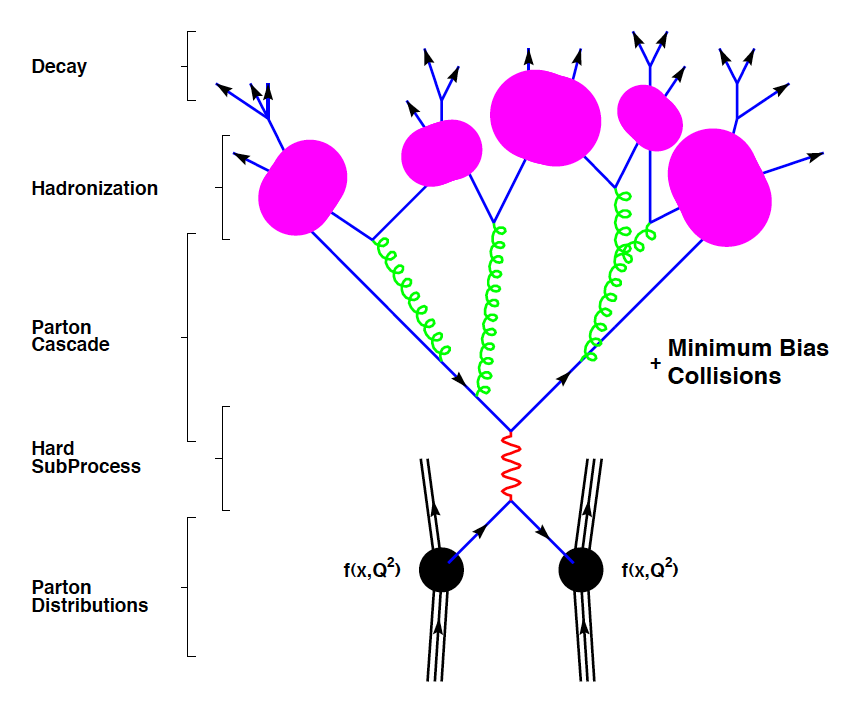
\includegraphics[width=0.75\textwidth]{images/EventProcess.png}
  	\caption[Event Process in a Hadron Collision]
   	{The basic simulation structure for an event in a hadron collision including parton distribution, hard subprocess, parton showering, hadronization, final decay and pileup (Minimum Bias Collisions) \cite{GuidebookOfMcGenerators}.}
	\label{fig:EventProcess}
\end{figure}

For a lepton-lepton collider, the energies of the initial state leptons
is determined by the accelerator and is well known. For a
hadron-hadron collider each hadron is regarded as a collection
of quarks, antiquarks and gluons each of which carries
some fraction $x$ of the hadron's momentum at a scale $Q$ with a 
number density $f(x,Q^{2})$. $Q$ characterizes the hard scattering 
($Q^{2}=M^{2}_{l^{+}l^{-}}, p_{T}^{2}$, ect.)
and changes on the order of $O(1)$ are equivalent\cite{Campbell:2006wx}. 
%In a proton-proton interaction a parton is resolved
%at scale $Q$ and momentum fraction $x$ from each
%proton. 
Figure \ref{fig:EventProcess} 
shows a proton-proton collision where a valence quark
is separated from one of the colliding protons and a 
a sea anti-quark is separated from the other of the colliding protons.
The phenomenology of the parton interaction is encoded
in the parton distribution function $f(x,Q^{2})$. 
The parton distribution function represents the probability
densities to find a parton carrying
a momentum faction $x$ at a squared energy
scale $Q^{2}$\cite{Martin:2009iq}. 
Since the hadronization scale is much smaller than the hard scale the impact
of the hadronization model choice on the final state is typically
small for most physics analyses. 
%Parton showers are essential in providing the %%exclusive?
%description of the event: at leading order the transverse momentum
%for the $W$ will always be zero since there is nothing for the $W$
%to recoil against.

The beam remnants are the colored remains of the proton which
are left behind when the parton which participates in the hard subprocess
is pulled out. As the beam remnants are color connected to the hard
subprocess they should be included in the hadronization system. 
Multiple parton interactions (MPI) where more than one pair
of beam partons interact are also simulated. 
Due to the composite nature of hadrons and the low impact
parameter of spectator partons MPI
have an increase rate of occurrence in the presence of a 
hard scattering process. 
Figure \ref{DPSandSPS} shows a comparison of feynman diagrams for W+jj interaction from 
double parton scattering (an MPI interaction) and single parton scattering. 
In the $\Wbb$ analysis the effects from double parton scattering must be taken into 
account when calculating the measured cross section. 
MPI agreement between data and simulation is tested 
by observing the relative $p_{T}$ balance of the two 
jets via the ratio of $(p_{T,j_{1}}+p_{T,j_{2}})/p_{T,j_{1},j_{2}}$ \cite{Chatrchyan:2013xxa}.

\begin{figure}[hb]
\centering
  \begin{subfigure}[b]{.475\textwidth}
	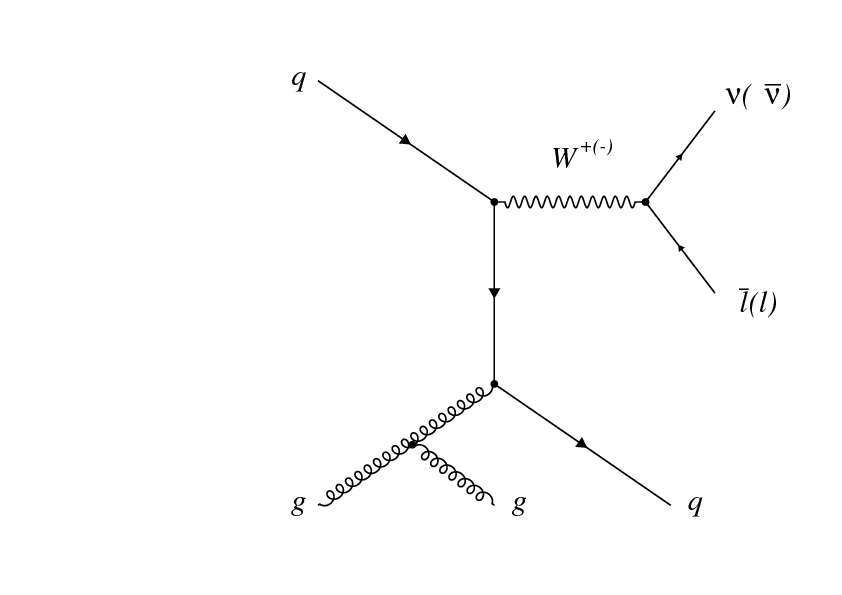
\includegraphics[trim = 0mm 0mm 0mm 0mm, clip,width=\textwidth]{images/figs_SPS_final.png}
	\end{subfigure}	
   \begin{subfigure}[b]{.475\textwidth}
	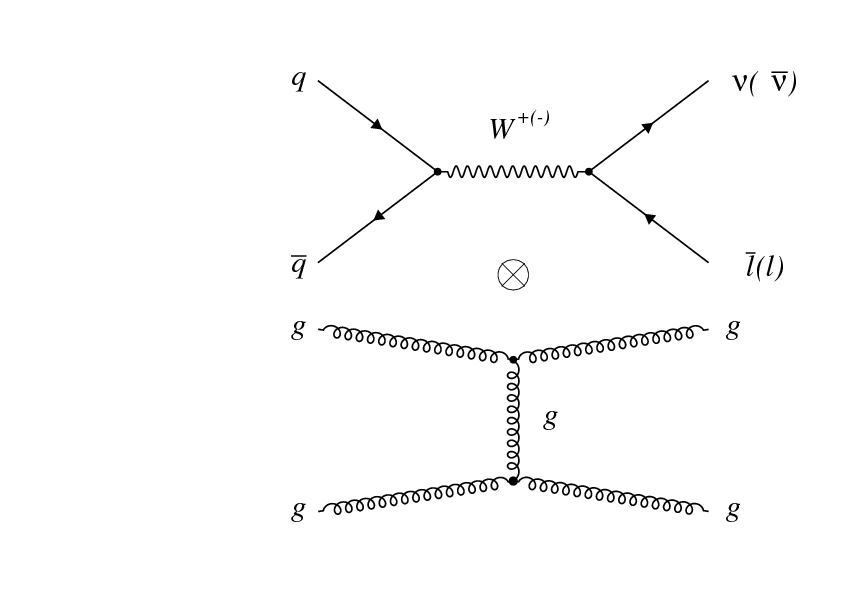
\includegraphics[trim = 0mm 0mm 0mm 0mm, clip,width=\textwidth]{images/figs_DPS_final.png}
    \end{subfigure}	
  \caption[]
   	{Single Parton Scattering and Double Parton Scattering in a W+jj event}
    \label{fig:DPSandSPS}
\end{figure}

The LHC is a high luminosity experiment. Therefore, 
an obseved event will have, as background, interactions from other colliding protons.
Successful event simulation must include  
pileup from other proton-proton collisions.
%b quarks are not expected to be
%produced at any signi�cant rate in nonperturbative processes [1], and they do not occur
%as valence �avours of the commonly used beam particles. A priori, they are therefore
%excellent probes of the underlying hard dynamics, whether that involves standard QCD
%processes or various kinds of new physics
\section{Monte Carlo Generator Programs}

\label{sec:MCGenerators}
A number of monte carlo (MC) generators are used to simulate
physics processes. The MC method makes use of a random
number generator to simulate event to event fluctuations
which are intrinsic quantum processes. 
The choice of MC generator is largely dependent on the 
type of process to be simulated. %fix
%K-factors
\subsection{MadGraph}
MadGraph\cite{Alwall:2007st} is is a matrix element generator for SM processes at
any collider. It provides a computation of tree-level matrix elements
with a fixed number of partons in the final state. 
For a user-specified process MadGraph generates
the amplitudes for all relevant subprocesses and produces
the mappings for the integration over the phase space. 
The final state only events may be passed directly to a shower MC program.
\subsection{Tauloa}
Tauloa\cite{TAUOLA} is a package which is used for generation of tau lepton decays including
spin polarization. For each tau decay mode there is a individual phase space generator,
modeling of the weak decay including first order QED corrections for leptonic decays
and a part describing the hadronic current.
\subsection{PYTHIA}
At leading order $\mathtt{PYTHIA}$\cite{Pythia} 
contains approximately 240 different $2\rightarrow n$ subprocesses.
The initial state shower is based on backwards evolution whereby the 
hard scattering process is simulated and is evolved backwards in time to the shower
initiators. Partons radiated in the initial state can initiate final-state showers
of their own. The Lund string model is used in hadronization; it is based on linear confinement
where quarks  are located at the ends of the string and gluons
are energy and momentum carrying kinds in the string. The production of a new $q\bar{q}$
pair causes the string to break. A quark from one break can combine with an antiquark
from an adjacent quark to form a meson. 
\subsection{MCFM}%reread carefully
Monte Carlo for FeMtobarn (MCFM)\cite{MCFM} processes at hadron 
colliders is a parton-level Monte Carlo
program which gives next to leading order predictions for 
a range of processes at hadron colliders. The difference between leading and 
next to leading order is described in section \ref{sec:SMSection}.
 MCFM
produces weighted events and therefore can
give very accurate predictions for event rates at NLO with cuts included, 
however it gives very little information about regions of phase space which are 
dominated by multiple parton interactions. 
Since the final state contains partons rather than hadrons, full detector simulation cannot
be performed using the MCFM output. Furthermore, a parton to hadron correction factor
must be included when comparing (for instance) with \PYTHIA, a generator which does
include hadrons in the final state. The parton to hadron correction factor is estimated
for the $\Wbb$ cross section measurement detailed later in this thesis and is shown to give significant
correction to the overall simulated cross section. 
%ref http://mcfm.fnal.gov/mcfm.pdf
\section{Detector Simulation}
$\mathtt{GEANT4}$\cite{GEANT4} is a toolkit for simulating the passage of
photons, muons, electrons, hadrons and ions through matter at energies from 250 eV to 
several PeV. The simulation package models the 
detector geometry, electric and magnetic fields and a wide range 
of initial to final state physics processes.
Geometry simulation includes a detailed model of the experiment
including layout of the detectors and the location of absorbers (cables, cooling systems, ect.)
Run management for recording details of each run as well as
a number of options for the visualization of the simulation output.
Magnetic field simulation makes use of detailed measurements of 
the magnetic field throughout the CMS detector.
$\mathtt{GEANT4}$ uses decay tables for to properly simulate decay rates 
for particles such as $\pi$, $K$ mesons
and resonant baryons based on data from the Particle Data Group\cite{PhysRevD.86.010001}.
The models used for decay of various physics processes are either
theory or data driven and the toolkit offers a large variety of complementary
and sometimes alternative physics models. 
%need transition sentencce
The probability of a particle surviving a distance $l$ 
\begin{equation}
P(l)=e^{-\eta_{\lambda}}
\end{equation}
where $\eta_{\lambda}$ is an exponential distribution which is independent of 
material and energy; therefore, $\eta_{\lambda}=-\ln(\eta)$ and $\eta$ is
a random number on the interval $(0,1)$. \GEANTfour has been an essential and 
very successful tool in the simulation of detector effects at CMS.